%%%%%%%%%%%%%%%%%%%%%%%%%%%%%%%%%%%%%%%%%
% Beamer Presentation
% LaTeX Template
% Version 1.0 (10/11/12) 
%
% This template has been downloaded from:
% http://www.LaTeXTemplates.com
%
% License:
% CC BY-NC-SA 3.0 (http://creativecommons.org/licenses/by-nc-sa/3.0/)
%
%%%%%%%%%%%%%%%%%%%%%%%%%%%%%%%%%%%%%%%%%

%----------------------------------------------------------------------------------------
%	PACKAGES AND THEMES
%----------------------------------------------------------------------------------------

\documentclass{beamer}

\mode<presentation> {
%\mode<handouts> {
%\mode<article> {


% The Beamer class comes with a number of default slide themes
% which change the colors and layouts of slides. Below this is a list
% of all the themes, uncomment each in turn to see what they look like.


%\usetheme{default}
%\usetheme{AnnArbor}
%\usetheme{Antibes}
%\usetheme{Bergen}
%\usetheme{Berkeley}
%\usetheme{Berlin}
%\usetheme{Boadilla}
\usetheme{CambridgeUS}
%\usetheme{Copenhagen}
%\usetheme{Darmstadt}
%\usetheme{Dresden}
%\usetheme{Frankfurt}
%\usetheme{Goettingen}
%\usetheme{Hannover}
%\usetheme{Ilmenau}
%\usetheme{JuanLesPins}
%\usetheme{Luebeck}
%\usetheme{Madrid}
%\usetheme{Malmoe}
%\usetheme{Marburg}
%\usetheme{Montpellier}
%\usetheme{PaloAlto}
%\usetheme{Pittsburgh}
%\usetheme{Rochester}
%\usetheme{Singapore}
%\usetheme{Szeged}
%\usetheme{Warsaw}

% As well as themes, the Beamer class has a number of color themes
% for any slide theme. Uncomment each of these in turn to see how it
% changes the colors of your current slide theme.

%\usecolortheme{albatross}
\usecolortheme{beaver}
%\usecolortheme{beetle}
%\usecolortheme{crane}
%\usecolortheme{dolphin}
%\usecolortheme{dove}
%\usecolortheme{fly}
%\usecolortheme{lily}
%\usecolortheme{orchid}
%\usecolortheme{rose}
%\usecolortheme{seagull}
%\usecolortheme{seahorse}
%\usecolortheme{whale}
%\usecolortheme{wolverine}

%\setbeamertemplate{footline} % To remove the footer line in all slides uncomment this line
%\setbeamertemplate{footline}[page number] % To replace the footer line in all slides with a simple slide count uncomment this line

%\setbeamertemplate{navigation symbols}{} % To remove the navigation symbols from the bottom of all slides uncomment this line
}

\usepackage{graphicx} % Allows including images
\graphicspath{{../figures}}
\usepackage{booktabs} % Allows the use of \toprule, \midrule and \bottomrule in tables
\usepackage{amsmath, amssymb, amsthm, gensymb,mathrsfs}%,eufrak}
\usepackage{hyperref}
\usepackage{tabularx}
\usepackage{longtable}
\usepackage{makecell}
\usepackage{multicol}
\usepackage{physics}

\newcommand{\uvec}[1]{\textbf{#1}}

\newcounter{excounter}
%\renewcommand{\thefpcounter}{\thechapter.\arabic{fpcounter}}
%\renewcommand{\thefpcounter}{\thesection.\arabic{fpcounter}}
\renewcommand{\theexcounter}{\arabic{excounter}}

\newtheorem{teorema}{Teorema}[section]
\newtheorem{definicio}{Definició}[section]

\usepackage[lastexercise]{exercise}

\graphicspath{{../figures}}

%----------------------------------------------------------------------------------------
%	 TITLE PAGE
%----------------------------------------------------------------------------------------

\title[Monte Carlo Methods]{Unsupervised learning} % The short title appears at the bottom of every slide, the full title is only on the title page

\author{Jordi Villà i Freixa} % Your name
\institute[FCTE] % Your institution as it will appear on the bottom of every slide, may be shorthand to save space
{
Universitat de Vic - Universitat Central de Catalunya \\
Study Abroad\\ % Your institution for the title page
\medskip
\textit{jordi.villa@uvic.cat} % Your email address
}
%\date{\today} % Date, can be changed to a custom date
\date{course 2023-2024}
\logo{
\includegraphics[width=.1\textwidth]{FCTE}}
\begin{document}

\begin{frame}
\titlepage % Print the title page as the first slide
\end{frame}

\begin{frame}
\frametitle{Índex} % Table of contents slide, comment this block out to remove it
\tableofcontents % Throughout your presentation, if you choose to use \section{} and \subsection{} commands, these will automatically be printed on this slide as an overview of your presentation
\end{frame}

%----------------------------------------------------------------------------------------
%	PRESENTATION SLIDES
%----------------------------------------------------------------------------------------
\section{Introduction and scope}
\begin{frame}
  \frametitle{Preliminary note}
  The material in these slides is strongly based on \cite{kroese2020}. When other materials are used, they are cited accordingly.

  Mathematical notation follows as good as it can a \href{https://ctan.math.utah.edu/ctan/tex-archive/macros/latex/contrib/mlmath/mlmath.pdf}{good practices proposal} from the Beijing Academy of Artificial Intelligence.
  \end{frame}

%------------------------------------------------
\section{Introduction} % Sections can be created in order to organize your presentation into discrete blocks, all sections and subsections are automatically printed in the table of contents as an overview of the talk
%------------------------------------------------

%\subsection{Subsection Example} % A subsection can be created just before a set of slides with a common theme to further break down your presentation into chunks

\begin{frame}{What to expect?}
  In this session we will discuss:
  \begin{itemize}
    \item Unsupervised learning
    \item The Expectation-Maximization Algorithm
    \item Principal component analysis
  \end{itemize}
\end{frame}

\section{Unsupervised learning}

\begin{frame}{Unsupervised learning}
    \begin{figure}
        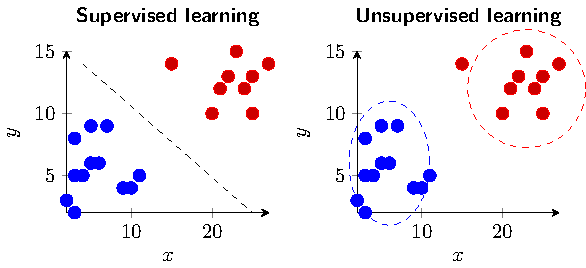
\includegraphics[width=0.7\linewidth]{supervised_unsupervised}
        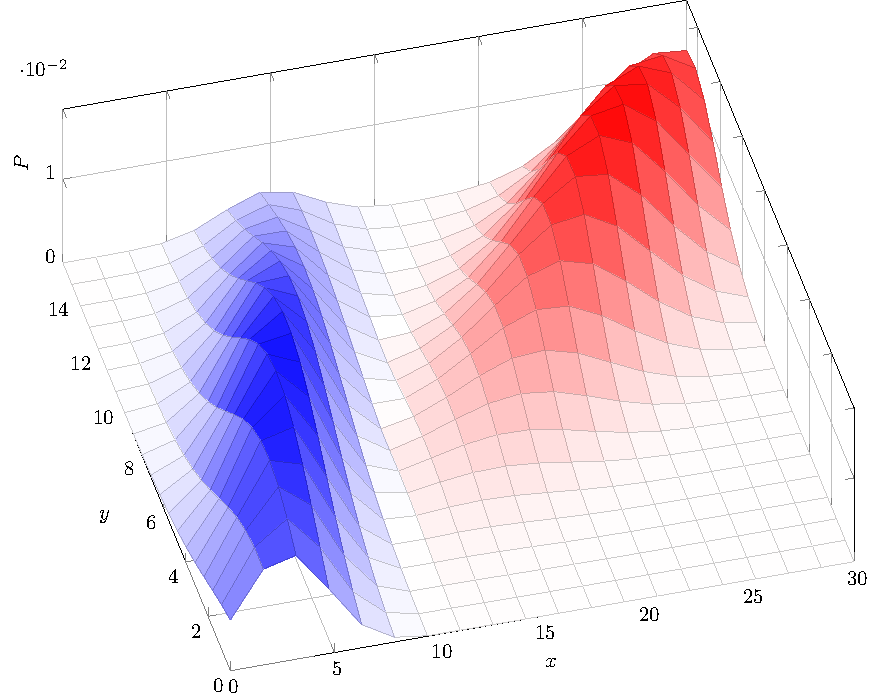
\includegraphics[width=0.3\linewidth]{2dbivariate}
        \caption{Supervised-unsupervised learning, and actual pdf behind the data}
        \label{fig:supunsup}
    \end{figure}
\end{frame}

\begin{frame}{Generating data}
    \begin{Exercise}{Generate bivariate data}
        Generate data from a collection of three different bivariate distributions with arbitrary means and covariances.
    \end{Exercise}
\end{frame}


\begin{frame}{Joint probability distribution}
    \begin{figure}
        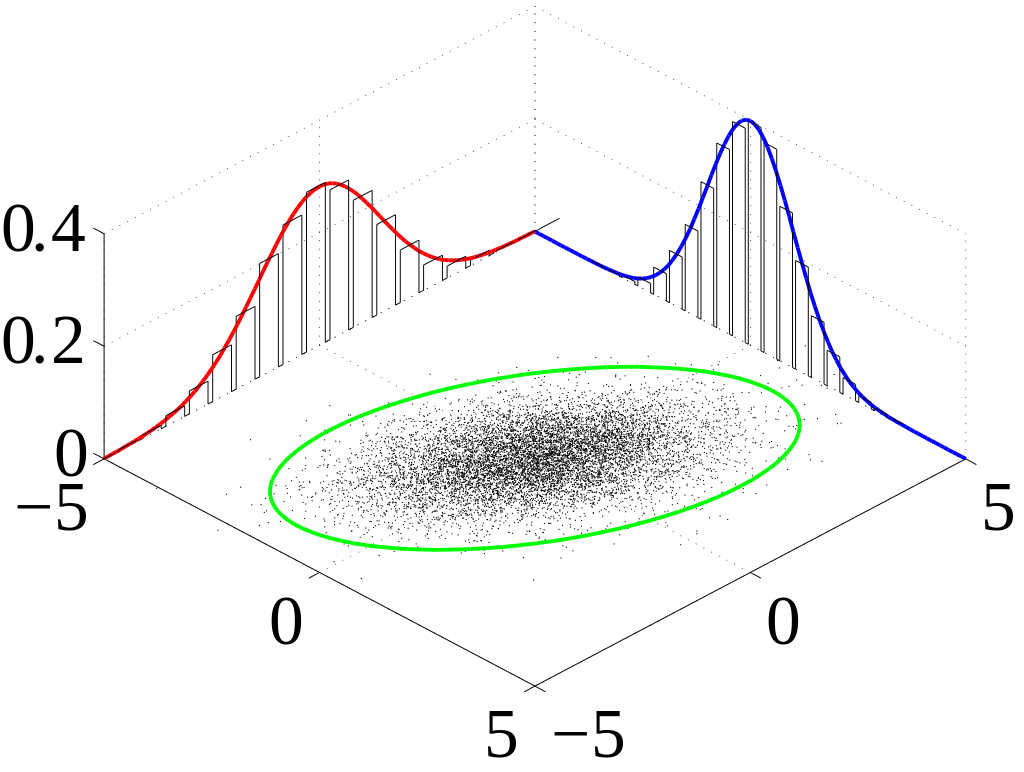
\includegraphics[width=0.6\linewidth]{Multivariate_normal_sample}
        \caption{\href{https://commons.wikimedia.org/wiki/File:Multivariate_normal_sample.svg}{Multivariate normal sample}}
    \end{figure}
\end{frame}

\section{MLE vs EM}
\begin{frame}{Maximum likelihood and Expectation-Maximization algorithm}
    We already saw how to use the K-means algorithm, based on the {\em distances} of the different data points. Now we will use another method that is based on assuming a given distribution of the data. 
    \\[10pt]
    Maximum likelihood estimation (MLE) is an approach to density estimation for a dataset by searching accross probability distributions and their parameters. However, it needs that {\em latents} (or hidden) variables not to exist in the training dataset. It requires the dataset to be complete, or fully observed: that all variables that are relevant to the problem are present.
    \\[10pt]
    The {\bf expectation-maximization (EM)} algorithm is an approach for performing MLE when latent variables are present. It is common to use it in estimating the density when data is missing, such as clustering in the {\bf Gaussian Mixture Model}.
\end{frame}

\begin{frame}{The EM algorithm}
    Let us assume a {\em mixture model}: unspecified combinadtion of multiple probability distribution functions. In our case, we will deal with the {\em Gaussian mixture model (GMM)}, where the parameters to estimate are the mean and the standard deviation for each Gaussian (normal) distribution in the mixture.
    \begin{enumerate}
        \item E-step: Estimate the missing variables in the dataset: the expected value for each latent variable.
        \item M-step: Maximize the parameters of the model in the presence of the data, using MLE.
    \end{enumerate}
\end{frame}

\begin{frame}[fragile]{A one dimensional example for EM}
    Adapted from \href{https://machinelearningmastery.com/expectation-maximization-em-algorithm/}{here}
    \begin{lstlisting}
# example of a bimodal constructed from two gaussian processes
from numpy import hstack
from numpy.random import normal
from matplotlib import pyplot
# generate a sample
X1 = normal(loc=20, scale=5, size=3000)
X2 = normal(loc=40, scale=5, size=7000)
X = hstack((X1, X2))
# plot the histogram
pyplot.hist(X, bins=50, density=True)
pyplot.show()
    \end{lstlisting}
\end{frame}

\begin{frame}{A one dimensional example for EM}
    \begin{figure}
        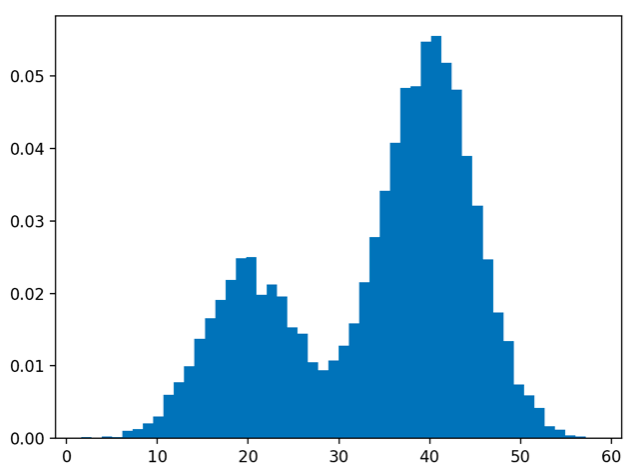
\includegraphics[width=0.7\linewidth]{hist}
    \end{figure}
\end{frame}

\begin{frame}[fragile]{A one dimensional example for EM}
    \small
    \begin{lstlisting}
from numpy import hstack
from numpy.random import normal
from sklearn.mixture import GaussianMixture
# generate a sample
X1 = normal(loc=20, scale=5, size=3000)
X2 = normal(loc=40, scale=5, size=7000)
X = hstack((X1, X2))
# reshape into a table with one column
X = X.reshape((len(X), 1))
# fit model
model = GaussianMixture(n_components=2, init_params='random')
model.fit(X)
yhat = model.predict(X) # predict latent values
print(yhat[:100])       # check latent value for first few points
print(yhat[-100:])      # check latent value for last few points
    \end{lstlisting}
    \normalsize
\end{frame}

\begin{frame}{The maths behind}
    \[\mu_k = \frac{\sum_{i=1}^n p_i^{(t)}(k)\uvec{x}_i}{\sum_{i=1}^n p_i^{(t)}(k)}\]

    \[\mathrm{Cov}_k=\frac{\sum_{i=1}^n p_i^{(t)}(k)(\uvec{x}_i-\mu_k)(\uvec{x}_i-\mu_k)^T}{\sum_{i=1}^n p_i^{(t)}(k)}\]

    where we estimate the pdf by using the previous iteration expectation and covariace:

    \[p_i^{(t)}(k) \varpropto w_k^{(t-1)} \phi_k(\uvec{x}_i | \mu_k^{(t-1)},\mathrm{Cov}_k^{(t-1)})\]
\end{frame}

\section{Principal Component Analysis}

\begin{frame}{\href{https://builtin.com/data-science/step-step-explanation-principal-component-analysis}{PCA}}
    \begin{enumerate}
        \item Get some data
        \item Substract the mean from each data dimension. Better standardize: $z=\frac{\uvec{x}-\bar{\uvec{x}}}{\sigma}$. Calculate the covariance matrix $X X^T$.
        \item Diagonalize and obtain unit eigenvectors $c^T X X^T c -\lambda c^T c$ via SVD: $X X^T=U D^2 U$
        \item Choosing components and forming a feature vector 
        \item Recast the data along the chosen PC axes. $\uvec{x}_i^{\mathrm{PC}}=U_k U_k^T \uvec{x}_i$
    \end{enumerate}
    \begin{figure}
        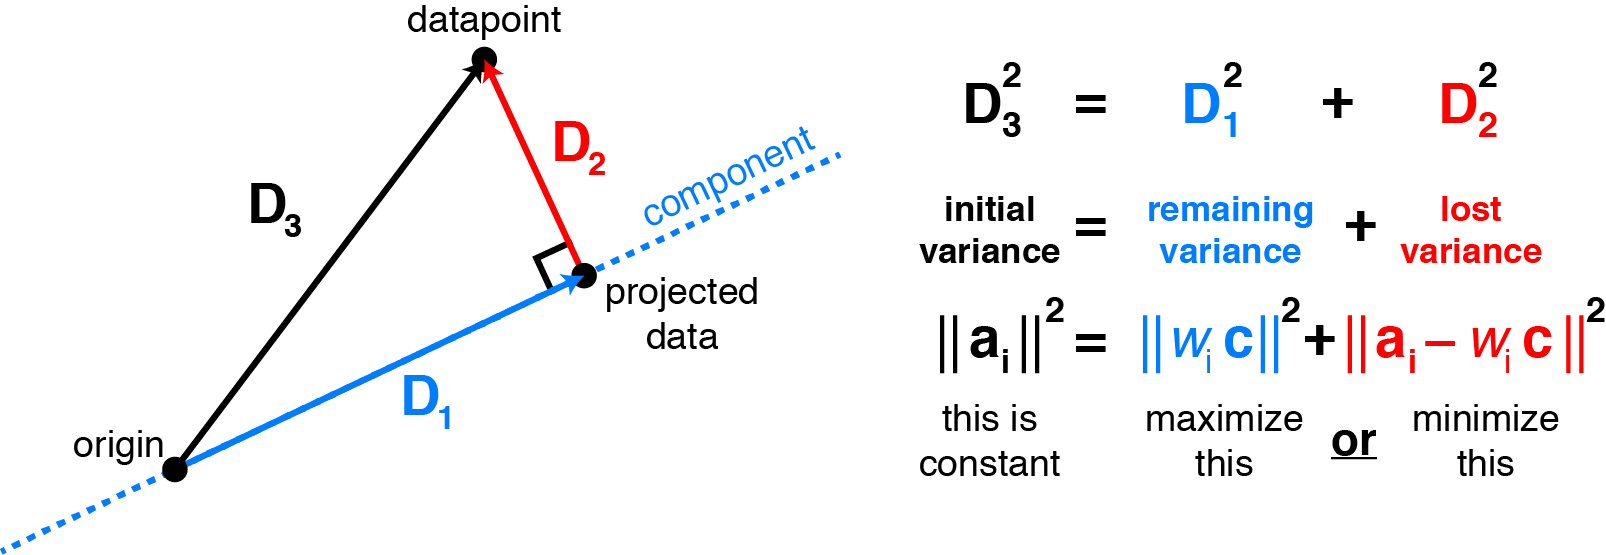
\includegraphics[width=0.7\linewidth]{projection_intuition}
        \caption{Maximizing variance in principal component space is equivalent to minimizing least-squares reconstruction error. Taken from \href{http://alexhwilliams.info/itsneuronalblog/2016/03/27/pca/}{this post}}
    \end{figure}
\end{frame}

\begin{frame}{EX2}
    \begin{Exercise}{EX2. PCA example}
        Get the {\em Iris} dataset from the \href{https://archive.ics.uci.edu}{UCI repository}. 
        \begin{enumerate}
            \item Using the {\bf kdeplot} method of {\bf seaborn}, generate a figure for the kernel density plots of the variable {\em Petal.length} for each of the three species of {\em Iris sp.} in the dataset.
            \item Show a scatter plot of the variable Petal.length vs the variable Sepal.length and comment on the correlation you see. 
            \item In order to analyze the possible correlatoons between the different data in the file, perform a PCA and obtain the principal component matrix $U$ as well as the diagonal matrix $D^2$. What can you say in terms of the variance?
            \item Project the data on the first component and plot the kernel density estimate of the PCA-combined data. 
        \end{enumerate}
    \end{Exercise}
\end{frame}

\section{Bibliography}
\bibliographystyle{unsrt}
\bibliography{DataSciencewithPython}
\end{document}